\section{Introduction}\label{sec:intro}

\subsection{Towards a Decentralized Application Stack}

The introduction of Bitcoin \cite{nakamoto2009bitcoin} has triggered a new wave of decentralization in computing. 
Bitcoin illustrated a novel set of benefits: decentralized control, where ``no one'' owns or controls the network; immutability,
where written data is tamper-resistant (``forever''); and the ability to create \& transfer assets on the network, without reliance on a central entity.

The initial excitement surrounding Bitcoin stemmed from its use as a token of value, for example as an alternative to government-issued currencies.
As people learned more about the underlying blockchain technology, they extended the scope of the technology itself (e.g. smart contracts), as well as applications (e.g. intellectual property).

With this increase in scope, single monolithic ``blockchain'' technologies are being re-framed and refactored into building blocks at four levels of the stack:
\begin{enumerate}
 \item Applications
 \item Decentralized computing platforms (``blockchain platforms'')
 \item Decentralized processing (``smart contracts'') and decentralized storage (file systems, databases), and decentralized communication
 \item Cryptographic primitives, consensus protocols, and other algorithms
\end{enumerate}

\subsection{Blockchains and Databases}
We can frame a traditional blockchain as a database (DB), in the sense that it provides a storage mechanism.
If we measure the Bitcoin blockchain by traditional DB criteria, it’s terrible: throughput is just a few transactions per second (tps), latency before a single confirmed write is 10 minutes, and capacity is a few dozen GB.
Furthermore, adding nodes causes more problems: with a doubling of nodes, network traffic quadruples with no improvement in throughput, latency, or capacity.
It also has essentially no querying abilities: a NoQL\footnote{We are introducing the term NoQL to describe a database with essentially no query abilities. This term is not to be confused with the database company noql (\url{http://www.noql.com}).} database.

In contrast, a modern distributed DB can have throughput exceeding 1 million tps, capacity of petabytes and beyond, latency of a fraction of a second, and throughput and capacity that increases as nodes get added.
Modern DBs also have rich abilities for insertion, queries, and access control in SQL or NoSQL flavors; in fact SQL is an international ANSI and ISO standard.

\subsection{The Need for Scale}
Decentralized technologies hold great promise to rewire modern financial systems, supply chains, creative industries, and even the Internet itself.
But these ambitious goals need scale: the storage technology needs throughput of up to millions of transactions per second (or higher), sub-second latency\footnote{It takes light 140 ms to make one trip around the world, or 70 ms halfway around. Some financial applications need 30-100 ms latency, though due to speed-of-light constraints those necessarily need to be more locally constrained. Section \ref{sec:latency} explores this in detail.}, and capacity of petabytes or more.
These needs exceed the performance of the Bitcoin blockchain by many orders of magnitude.

\subsection{BigchainDB : Blockchains Meet Big Data}
This paper introduces BigchainDB, which is for database-style decentralized storage: a blockchain database.
BigchainDB combines the key benefits of distributed DBs and traditional blockchains, with an emphasis on scale, as Table \ref{tab:bigchain_comparison} summarizes.

\begin{table}[h]
  \caption{BigchainDB compared to traditional blockchains, and traditional distributed DBs}
  \footnotesize
  \makebox[\textwidth][c]{
  \centering
  \setlength\extrarowheight{3pt}
  \begin{tabular}{ | m{\dimexpr 0.25\linewidth-2\tabcolsep} |
	  M{\dimexpr 0.25\linewidth-2\tabcolsep} |
	  M{\dimexpr 0.25\linewidth-2\tabcolsep} |
	  M{\dimexpr 0.25\linewidth-2\tabcolsep} |} \Xhline{4\arrayrulewidth}\rowcolor{black}
  				                  & \color{white} Traditional Blockchain & \color{white} Traditional Distributed DB & \color{white} BigchainDB \\\Xhline{4\arrayrulewidth}
  High Throughput; increases with nodes$\uparrow$ & - 		           & \checkmark                  & \checkmark          \\\hline
  Low Latency                                     & - 		           & \checkmark                  & \checkmark          \\\hline
  High Capacity; increases with nodes$\uparrow$   & - 		           & \checkmark                  & \checkmark          \\\hline
  Rich querying                                   & - 		           & \checkmark                  & \checkmark          \\\hline
  Rich permissioning                              & - 		           & \checkmark                  & \checkmark          \\\hline
  Decentralized control                           & \checkmark 		   & -                          & \checkmark          \\\hline
  Immutability                                    & \checkmark 		   & -                          & \checkmark          \\\hline
  Creation \& movement of digital assets          & \checkmark 		   & -                          & \checkmark          \\\hline
  Event chain structure				  & Merkle Tree            & - 				& Hash Chain          \\
  \Xhline{4\arrayrulewidth}
  \end{tabular}
  }
  \label{tab:bigchain_comparison}
\end{table}

We built BigchainDB on top of an enterprise-grade distributed DB, from which
BigchainDB inherits high throughput, high capacity, low latency, a full-featured efficient NoSQL query language, and permissioning.
Nodes can be added to increase throughput and capacity.

\begin{figure}[!ht]
  \centering
  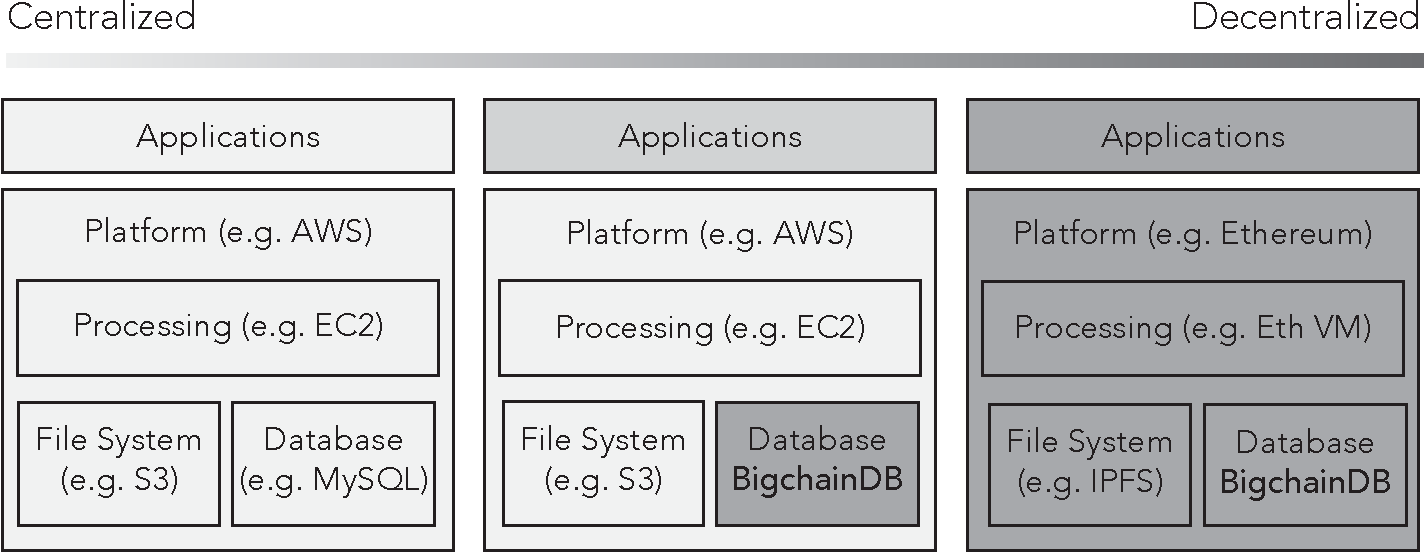
\includegraphics[width=\textwidth]{figure_1.pdf}
  \caption{From a base context of a centralized cloud computing ecosystem (left), BigchainDB can be added as another database to gain some decentralization benefits (middle).
  It also fits into a full-blown decentralization ecosystem (right).}
  \label{fig:bigchain_ecosystem}
\end{figure}

BigchainDB has the blockchain benefits of decentralized control, immutability, and creation \& transfer of assets.
The decentralized control is via a federation of nodes with voting permissions, that is, a super-peer P2P network \cite{ozsu2011principles}.
The voting operates at a layer above the DB’s built-in consensus.
Immutability / tamper-resistance is achieved via several mechanisms: shard replication, reversion of disallowed updates or deletes, regular database backups, and cryptographic signing of all transactions, blocks \& votes. Each vote on a block also includes the hash of a previous block (except for that block's votes).
Any entity with asset-issuance permissions can issue an asset; an asset can only be acquired by new owners if they fulfill its cryptographic conditions.
This means hackers or compromised system admins cannot arbitrarily change data, and there is no single-point-of-failure risk.

Scalable capacity means that legally binding contracts and certificates may be stored directly on the blockchain DB.
The permissioning system enables configurations ranging from private enterprise blockchain DBs to open, public blockchain DBs.
As we deploy BigchainDB, we are also deploying a public version.

\subsection{BigchainDB in the Decentralization Ecosystem}
Figure \ref{fig:bigchain_ecosystem} illustrates how BigchainDB can be used in a fully decentralized setting, or as a mild extension from a traditional centralized computing context.

BigchainDB is complementary to decentralized processing / smart contracts (e.g. Ethereum VM \cite{ethereum}\cite{buterin-ethereum} or Enigma \cite{enigma}\cite{zyskind2015enigma}), decentralized file systems (e.g. IPFS \cite{ipfs}), and communication building blocks (e.g. email).
It can be included in higher-level decentralized computing platforms (e.g. Eris/Tendermint \cite{eris}\cite{tendermint}).
It can be used side-by-side with identity protocols, financial asset protocols (e.g. Bitcoin \cite{nakamoto2009bitcoin}), intellectual property asset protocols (e.g. SPOOL \cite{dejonghe_spool}), and glue protocols (e.g. pegged sidechains \cite{back2010sidechains}, Interledger \cite{thomas2015interledger}).
Scalability improvements to smart contracts blockchains will help fully decentralized applications to better exploit the scalability properties of BigchainDB.

BigchainDB works with more centralized computing systems as well.
One use case is where decentralizing just storage brings the majority of benefit.
Another use case is where scalability needs are greater than the capabilities of existing decentralized processing technologies; in this case BigchainDB provides a bridge to an eventual fully-decentralized system.

\subsection{Contents}

This paper first gives background on related building blocks, with an eye to scale:
\begin{itemize}
 \item Section \ref{sec:background} - traditional blockchain scalability,
 \item Section \ref{sec:distributed} - distributed DBs, and
\end{itemize}


Then, this paper describes BigchainDB as follows:
\begin{itemize}
 \item Section \ref{sec:bigchaindb} - BigchainDB description,
 \item Section \ref{sec:implementation} - BigchainDB implementation, including capacity vs. nodes (Figure \ref{fig:bigchain_capacity_vs_nodes}),
 \item Section \ref{sec:latency} - BigchainDB latency analysis,
 \item Section \ref{sec:permissioning} - private vs. public BigchainDBs in a permissioning context,
 \item Section \ref{sec:benchmarks} - BigchainDB benchmarks, including throughput vs. nodes (Figure \ref{fig:bigchain_throughput_vs_nodes}),
 \item Section \ref{sec:deployment} - BigchainDB deployment, including use cases and timeline, and
 \item Section \ref{sec:conclusion} - conclusion.
\end{itemize}


The appendices contain:
\begin{itemize}
 \item Appendix \ref{appendix:glossary} - a glossary, e.g. clarifying “distributed” vs. “decentralized”,
 \item Appendix \ref{appendix:blockchain_scalability} - blockchain scalability proposals,
 \item Appendix \ref{sec:dns} - the Domain Name System (DNS), and
 \item Appendix \ref{appendix:benchmarks} – further BigchainDB benchmarks.
\end{itemize}